\begin{section}{Fish and their Swim Bladder}

    When immersed in water, fish experience the downward pull of gravity and the upward push of 
    buoyancy. Fish have developed key adaptations allowing them to move up and down in the water.
    There are several approaches to do this \cite{QUENTIN}, in this section we will consider fish
    with swim bladder as a mechanism for buoyancy only. Those fish have the ability modify their 
    own weight making themselves lighter to float up or heavier to sink down. They accomplish this
    by changing the amount of gas in an inner bladder without changing their volume. This bladder
    is known as \textbf{swim bladder}. Let's consider a simple model as shown in the picture 
    bellow where fish have a fixed volume $V$ and a density $\rho_p$ equiped with a swim bladder
    which can expand or compress changing its mass;
    
    \begin{center}
        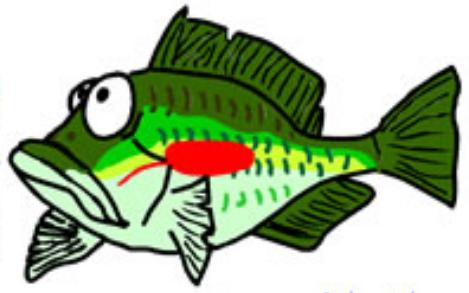
\includegraphics[scale=0.35]{./pics/fish_bladder.jpg}
    \end{center}
    
    In this model fish have a non constant density since its mass changes depending on the gas
    input/output in their swim bladder. Then the mass of fish can be written as the sum of a mass 
    $m_0$, related to the mass of its body without taking into account the gas inside their swim 
    bladder, and the mass $m_b$ inside their swim bladder. Mass $m_0$ can be regarded as fixed 
    since it doesn't change in the scale of time the mass $m_b$ varies, then for the density of 
    fish we have: 
    
    \begin{eqnarray}
        \rho_p &=& \frac{m_0 \pm m_b}{V}
        \nonumber\\
        {}&{}&{} \nonumber \\
        &=& \frac{m_0}{V} \pm \frac{m_b}{V}
         \nonumber\\
        {}&{}&{} \nonumber \\
        \label{fish_density}
        \rho_p &=& \rho_0 \pm \rho_b.
    \end{eqnarray}
    
    Equation (\ref{fish_density}) describes the mechanism allowing fish to modify their density in
    terms of the swim bladder, and then as we saw previously, this process might result in fish 
    floating up, being at rest at a given depth or sinking down without additional efforts. We can go 
    even further if we in addition consider equation (3.3),
    
    \begin{eqnarray}
        a &=& \left( \frac{\rho_{\omega}}{\rho_p} -1 \right)g,
        \nonumber\\
        {}&{}&{}
        \nonumber \\
        &=& \left( \frac{\rho_{\omega}}{\rho_0 \pm \rho_b} -1 \right)g,
        \nonumber\\
        {}&{}&{}
        \nonumber \\
        \label{fish_dynamics_00}
        &=& \left( \frac{1}{\frac{\rho_0}{\rho_{\omega}} \pm \frac{\rho_b}{\rho_{\omega}}} -1 \right)g.
    \end{eqnarray}
    
    Usually the density $\rho_0$ of fish is similar to the density of water \cite{QUENTIN}, then
    $\rho_{\omega} \simeq \rho_0$ and equation (\ref{fish_dynamics_00}) can be rewritten as follows:
    
    \begin{equation}
        \label{fish_dynamics_01}
        a = \left( \frac{1}{ 1 \pm \frac{\rho_b}{\rho_0}} - 1 \right)g.
    \end{equation}
    
    This last equation can be reduced if we use the next formula:
    
    \begin{equation}
        \label{formula}
        \frac{1}{1 \pm x} = 1 - \left(\pm x\right), \hspace{3mm} \text{for  $0<x<<1$ },
    \end{equation}
    since: $$\frac{\rho_b}{\rho_0} = \frac{m_b}{m_0} << 1. $$ Then equation (\ref{fish_dynamics_01})
    is equivalent to:
    
    \begin{equation}
        \label{fish_dynamics_02}
        a = - \left(\pm \frac{\rho_b}{\rho_0} g \right).
    \end{equation}
    
    The model we are considering show us the phenomelogy discussed in section \textbf{(II)} is a direct
    consequence of the mass amount in the swim bladder, which is essentially what happens in reality
    \cite{QUENTIN}.
    
\end{section}
